\documentclass[conference]{IEEEtran}
\IEEEoverridecommandlockouts
% The preceding line is only needed to identify funding in the first footnote. If that is unneeded, please comment it out.
\usepackage{cite}
\usepackage{amsmath,amssymb,amsfonts}
\usepackage{algorithmic}
\usepackage{algorithm}
\usepackage{graphicx}
\usepackage{textcomp}
\usepackage{xcolor}
\usepackage{booktabs}
\usepackage{tikz}
\usetikzlibrary{positioning,arrows.meta,fit,backgrounds}
\usepackage{url}
\renewcommand{\topfraction}{0.9}
\renewcommand{\dbltopfraction}{0.9}
\renewcommand{\textfraction}{0.1}
\renewcommand{\floatpagefraction}{0.8}
\renewcommand{\dblfloatpagefraction}{0.8}
\setcounter{topnumber}{3}
\setcounter{dbltopnumber}{3}
\def\BibTeX{{\rm B\kern-.05em{\sc i\kern-.025em b}\kern-.08em
    T\kern-.1667em\lower.7ex\hbox{\sc e\kern-.125em x}}}

\newcommand{\tmx}{\ensuremath{\times}}
\renewcommand{\algorithmicrequire}{\textbf{Input:}}
\renewcommand{\algorithmicensure}{\textbf{Output:}}

% Second row of authors (as in the IEEE conference template on Overleaf)
\makeatletter
\newcommand{\linebreakand}{%
  \end{@IEEEauthorhalign}
  \hfill\mbox{}\par\vspace{10pt}
  \mbox{}\hfill\begin{@IEEEauthorhalign}
}
\makeatother

\begin{document}

\title{Memory Architectures of AI Inference Chips:\\
Cycle-Accurate Evaluation and Spectral\\ Access-Pattern Analysis}

% Author block removed for now (uncomment to restore):
% \author{\IEEEauthorblockN{Dr. Prabhu Prasad B M}
% \IEEEauthorblockA{\textit{Indian Institute of Information}\\
% \textit{Technology Dharwad}\\
% Dharwad, Karnataka, India
% % \\ email address or ORCID
% }
% \linebreakand
% \IEEEauthorblockN{G. V. Prajwal}
% \IEEEauthorblockA{\textit{Indian Institute of Information}\\
% \textit{Technology Dharwad}\\
% Dharwad, Karnataka, India
% % \\ email address or ORCID
% }
% \and
% \IEEEauthorblockN{Siddhaartha B. S.}
% \IEEEauthorblockA{\textit{Indian Institute of Information}\\
% \textit{Technology Dharwad}\\
% Dharwad, Karnataka, India
% % \\ email address or ORCID
% }
% \and
% \IEEEauthorblockN{Yogeshgouda Patil}
% \IEEEauthorblockA{\textit{Indian Institute of Information}\\
% \textit{Technology Dharwad}\\
% Dharwad, Karnataka, India
% % \\ email address or ORCID
% }
% }
\author{}

\maketitle

\begin{abstract}
AI inference chips differ less in their arithmetic than in their memory systems. We evaluate seven memory-system archetypes (HBM GPUs, SRAM-plus-GDDR6 meshes, SRAM-plus-LPDDR5 NPUs, SRAM-only designs and a CPU baseline) on twelve AI inference scenarios and on eight SPEC CPU~2026 benchmarks, with one cycle-accurate DRAM model (Ramulator~2.1) underneath both. An operator-level model uses DRAM bandwidth measured per access pattern; an LLVM pass converts SPEC programs into L2-miss traces replayed on a common core; and every DRAM command is recorded to characterise the request stream at the memory controllers with its power spectral density (PSD). On batch-1 Llama-3.1 decode, SRAM-resident designs are 6.3--8.8\tmx{} faster than an HBM3 GPU, but the LPU-class design needs 76--654 chips and delivers 1/12--1/37 of the GPU's throughput per chip. Fast DRAM interfaces keep only 24--58\% of pin bandwidth on random accesses, against 86\% for DDR5. On general-purpose code the same memory systems reach only 0.32--0.83\tmx{} the IPC of a CPU with DDR5, because IPC follows last-level-cache latency. The PSD class of the request stream is set mainly by the program, not by the memory system.
\end{abstract}

\begin{IEEEkeywords}
AI accelerators, DRAM, HBM, SRAM, memory hierarchy, Ramulator, LLVM, SPEC CPU 2026, power spectral density
\end{IEEEkeywords}

%=====================================================================
\section{Introduction}
%=====================================================================
Large-language-model (LLM) inference is limited by data movement more than by arithmetic~\cite{wulf1995,gholami2024}: at batch~1, every generated token reads all weights and the key--value (KV) cache once. Chip designers have answered with very different memory systems. GPUs pair a modest cache with high-bandwidth memory (HBM)~\cite{choquette2023}; dataflow meshes and NPUs pair a large compiler-managed scratchpad with GDDR6 or LPDDR5~\cite{vasiljevic2021}; and SRAM-only designs such as the Groq LPU~\cite{abts2020} and the Cerebras wafer-scale engine~\cite{lie2023} keep all state on chip.

Datasheet bandwidth hides three effects. The bandwidth a DRAM system \emph{achieves} depends on the access pattern; the same memory systems must also run irregular, latency-bound general-purpose code; and \emph{how} requests arrive at the memory controllers determines how predictable memory access is~\cite{agarwal2025}. We study all three on one substrate. Our contributions are:
\begin{enumerate}
\item a reproducible framework that evaluates a chip's memory system, described in one configuration file, with cycle-accurate DRAM (Ramulator~2.1, the current release of Ramulator~2.0~\cite{luo2024}) on AI inference and on SPEC CPU~2026;
\item a per-access-pattern DRAM calibration feeding an operator-level placement, timing and energy model of inference;
\item an LLVM pass plugin and runtime that turn C/C++ programs into L2-miss traces, replayed on every memory system with an identical core;
\item a controller-level characterization that classifies the DRAM request stream by its PSD, extending the qualitative classes of~\cite{agarwal2025} with explicit thresholds and an anti-persistent class.
\end{enumerate}

%=====================================================================
\section{Related Work}\label{sec:related}
%=====================================================================
The memory wall~\cite{wulf1995} has become the main limit of transformer inference~\cite{gholami2024}. Pope~\emph{et~al.}~\cite{pope2023} model LLM inference across accelerators, and PagedAttention~\cite{kwon2023} turns KV reads into page gathers. LLMCompass~\cite{zhang2024} and GenZ~\cite{bambhaniya2024} model LLM inference hardware in more detail (operator mapping, parallelism strategies, interconnect topologies). Our operator model is simpler, a roofline~\cite{williams2009} per operator, but it uses DRAM bandwidth measured per access pattern instead of peak bandwidth; we do not compare against these frameworks quantitatively. AI accelerators range from the TPU's on-chip buffer plus DRAM~\cite{jouppi2017} to SRAM-only designs~\cite{abts2020,lie2023}; they are usually compared on vendor benchmarks, whereas we compare their \emph{memory systems} under one model. Ramulator~\cite{kim2016,luo2024} provides cycle-accurate DRAM models; we use it both to calibrate access patterns and as the back end of trace replay. SPEC suites have been characterised with binary instrumentation~\cite{luk2005} and hardware counters~\cite{limaye2018}; we instrument at the LLVM IR level~\cite{lattner2004}, inside the SPEC build harness. Finally, NoC traffic is known to be non-stationary and fractal~\cite{bogdan2010}, and Agarwal~\emph{et~al.}~\cite{agarwal2025} used the PSD of inter-arrival times at the memory controller to show how cache, buffer and network size change its predictability. We apply this analysis at the DRAM command level across five DRAM technologies.

%=====================================================================
\section{Problem Scenario and System Model}\label{sec:model}
%=====================================================================
\textbf{Problem.} An architect choosing the memory system of an inference chip needs to know the latency, chip count, throughput per chip and energy of inference; how much pin bandwidth each access pattern obtains; how the memory system serves general-purpose code; and how predictable the request stream is at the memory controllers. The SPEC study isolates the memory system behind one fixed core. The AI study instead compares complete chip classes: compute, link bandwidth and per-operator overhead differ between archetypes (Tables~\ref{tab:arch} and~\ref{tab:const}), so compute- and communication-bound results reflect the whole chip, not the memory system alone.

\textbf{Archetypes.} Table~\ref{tab:arch} lists the seven memory systems, with public-specification class values rather than vendor models. The key distinction is the role of the SRAM: a hardware \emph{cache} (CPU, GPU), a compiler-managed \emph{scratchpad} in front of DRAM (mesh, NPU), or \emph{resident} storage with no DRAM (LPU, wafer).

\begin{table*}[t]
\caption{Memory-System Archetypes (Public-Specification Class Values; TFLOPS = bf16 Peak)}
\label{tab:arch}
\centering
\footnotesize
\setlength{\tabcolsep}{2pt}
\begin{tabular}{@{}llllrrr@{}}
\toprule
Archetype & SRAM (role) & SRAM BW, latency & DRAM (ch.\,\tmx\,width, capacity, pin BW) & TFLOPS & Link GB/s & TDP W\\
\midrule
CPU + DDR5 & 96 MiB (cache) & 3 TB/s, 14 ns & DDR5-4800, 16\tmx32b, 512 GiB, 307 GB/s & 120 & 64 & 350\\
GPU + HBM3 & 50 MiB (cache) & 7 TB/s, 120 ns & HBM3 6.4\,Gb/s, 64\tmx64b, 80 GiB, 3,277 GB/s & 989 & 450 & 700\\
GPU + HBM4 & 128 MiB (cache) & 16 TB/s, 120 ns & HBM4 8\,Gb/s, 128\tmx64b, 288 GiB, 8,192 GB/s & 2,500 & 900 & 1,200\\
Mesh + SRAM + GDDR6 & 210 MiB (scratchpad) & 24 TB/s, 60 ns & GDDR6 14\,Gb/s, 8\tmx32b, 32 GiB, 448 GB/s & 370 & 400 & 300\\
NPU + SRAM + LPDDR5 & 144 MiB (scratchpad) & 12 TB/s, 40 ns & LPDDR5-6400, 8\tmx32b, 64 GiB, 205 GB/s & 200 & 32 & 75\\
LPU (SRAM only) & 230 MiB (resident) & 80 TB/s, 30 ns & none & 188 & 330 & 300\\
Wafer-scale SRAM & 44 GiB (resident) & 21,000 TB/s, 200 ns & none & 62,500 & 150 & 23,000\\
\bottomrule
\end{tabular}
\end{table*}

\textbf{Workloads.} The AI study covers Llama-3.1-8B and 70B~\cite{llama3} decode (batch 1 and 32, and a 32k-token context) and prefill, Mixtral-8x7B~\cite{jiang2024} decode, ResNet-50~\cite{he2016} and a DLRM-style recommender~\cite{naumov2019} with 64\,GB of embedding tables, all with 16-bit weights. The general-purpose study uses eight SPEC CPU~2026~\cite{spec2026} rate benchmarks with varied memory behaviour: stockfish, sqlite, omnetpp, sealcrypto, nest, marian, zstd and lbm.

\textbf{Memory model.} Each DRAM system is simulated in Ramulator~2.1 with one FR-FCFS~\cite{rixner2000}, open-row controller per channel. Consecutive 64\,B lines are interleaved across channels, and within a channel the MOP4CLXOR mapping spreads them over banks and rows. For SPEC, a common 4-wide, 4\,GHz out-of-order core runs in front of it, and the architecture's SRAM acts as the last-level cache (LLC) with its own capacity and the single latency of Table~\ref{tab:arch}. Power-of-two set counts round 210 and 230\,MiB to 208 and 232\,MiB, and the wafer's 44\,GiB is capped at a 1\,GiB LLC, which no trace outgrows. The SRAM-only designs reach a 2-channel DDR5 host memory for misses. This is an idealized sensitivity study: scratchpads and distributed tile memories are treated as a hardware-managed cache with one uniform, chip-scale latency and no software prefetching, so the SPEC results for the AI designs are an upper bound on their latency cost.

%=====================================================================
\section{Mathematical Formulation}\label{sec:math}
%=====================================================================
We define only the inference model and the metrics we report; DRAM and core timing come from Ramulator.

\textbf{Inference model.} For DRAM system $d$ and access pattern $p$, Ramulator measures the sustained bandwidth $B_d(p)$. Weights map to a sequential stream, KV reads to 4\,KiB page gathers, KV writes and activations to a 2:1 read/write stream, and embeddings to 256\,B row gathers. A model with persistent state $P$ and peak activations $A$ is spread over the fewest chips that hold it, with 90\% of the capacity $C$ per chip usable ($C$ is the DRAM capacity, or the SRAM capacity for SRAM-only designs):
\begin{equation}
n = \left\lceil \frac{P + A}{0.9\, C} \right\rceil .\label{eq:chips}
\end{equation}
A resident SRAM serves all bytes. A scratchpad holds activations (if they fit) and then as much persistent state as fits; everything else streams from DRAM. A cache serves persistent state only if all of it fits; GPU shared memory and hot-row caching (e.g.\ of skewed embedding tables) are not modelled. For mixture-of-experts models $P$ counts all experts, while traffic counts only the expected number of distinct active experts. One inference step executes the model's operators $o$ (matrix multiplications, attention, normalization) in order, each split across all $n$ chips (pure tensor parallelism). The step time is
\begin{equation}
T = \sum_{o} \Big[\max\big(t^{\mathrm{comp}}_o,\ t^{\mathrm{mem}}_o\big) + t^{\mathrm{comm}}_o + \tau\Big],\label{eq:step}
\end{equation}
with four terms per operator:
\begin{itemize}
\item $t^{\mathrm{comp}}_o = F_o/(n\,\Pi)$: the operator's FLOPs $F_o$, split over $n$ chips, at the chip's effective FLOP rate $\Pi$ (matrix peak times the efficiency in Table~\ref{tab:const}; half the vector peak for vector operators).
\item $t^{\mathrm{mem}}_o = \sum_p D_{o,p}/(n\,B_d(p))$: its DRAM bytes in each access pattern $p$, split over $n$ chips, each at the bandwidth \emph{measured for that pattern} rather than the datasheet bandwidth. SRAM bytes are timed the same way with the SRAM bandwidth; the SRAM and DRAM paths run in parallel and the slower one counts. SRAM latency is not modelled.
\item $t^{\mathrm{comm}}_o$: the collective after the operator when $n>1$. An all-reduce of $M$ bytes takes $2\lceil\log_2 n\rceil h + 2\frac{n-1}{n}\frac{M}{L}$, with hop latency $h$ and link bandwidth $L$~\cite{thakur2005}; embeddings use an all-to-all.
\item $\tau$: a fixed launch or synchronization overhead per operator (Table~\ref{tab:const}).
\end{itemize}
Compute and memory overlap, so the slower of the two sets the operator's time; this is a roofline~\cite{williams2009} per operator. At batch~1, for example, decode reads every weight once while doing little arithmetic, so $t^{\mathrm{mem}}$ dominates and $T$ is roughly the weight bytes divided by the measured stream bandwidth. The step is \emph{bound by} whichever of the four terms contributes most to $T$. Pure tensor parallelism over all $n$ chips is a simplification: at the 76--654 chips of the SRAM-only designs, real deployments combine it with pipeline parallelism, so our communication time is an upper bound. Energy per token counts the bits moved in SRAM, DRAM and links times their energy per bit (Table~\ref{tab:const}) plus 0.4\,pJ/FLOP; an upper bound with static power is $n\times\mathrm{TDP}\times T$ per token.

\begin{table}[t]
\caption{Inference-Model Constants per Archetype}
\label{tab:const}
\centering
\footnotesize
\setlength{\tabcolsep}{3pt}
\begin{tabular}{@{}lrrrrrr@{}}
\toprule
 & Matrix & $\tau$ & Hop $h$ & \multicolumn{3}{c}{Energy (pJ/bit)}\\
\cmidrule{5-7}
Archetype & eff. & ($\mu$s) & ($\mu$s) & SRAM & DRAM & Link\\
\midrule
CPU + DDR5 & 0.6 & 2 & 1.0 & 0.6 & 15 & 10\\
GPU + HBM3 & 0.7 & 3 & 0.8 & 0.8 & 3.9 & 5\\
GPU + HBM4 & 0.7 & 3 & 0.8 & 0.8 & 3.0 & 4\\
Mesh + GDDR6 & 0.6 & 2 & 1.5 & 0.3 & 7.5 & 8\\
NPU + LPDDR5 & 0.6 & 2 & 2.0 & 0.3 & 4.5 & 10\\
LPU (SRAM)$^\ast$ & 0.8 & 2 & 0.6 & 0.25 & -- & 4\\
Wafer (SRAM)$^\ast$ & 0.4 & 5 & 2.0 & 0.3 & -- & 8\\
\bottomrule
\end{tabular}\\[2pt]
\raggedright\scriptsize $^\ast\tau$ and $h$ tuned to published batch-1 token rates.
\end{table}

\textbf{SPEC metrics.} Each configuration runs $N$ and $2N$ instructions and the difference is reported, so the LLC is warm. We report IPC relative to CPU + DDR5 (geometric mean across benchmarks) and DRAM accesses per kilo-instruction after the LLC (APKI).

%=====================================================================
\section{Proposed Methodology}\label{sec:method}
%=====================================================================
Fig.~\ref{fig:framework} shows the framework. Only the memory system differs between architectures.

\begin{figure*}[t]
\centering
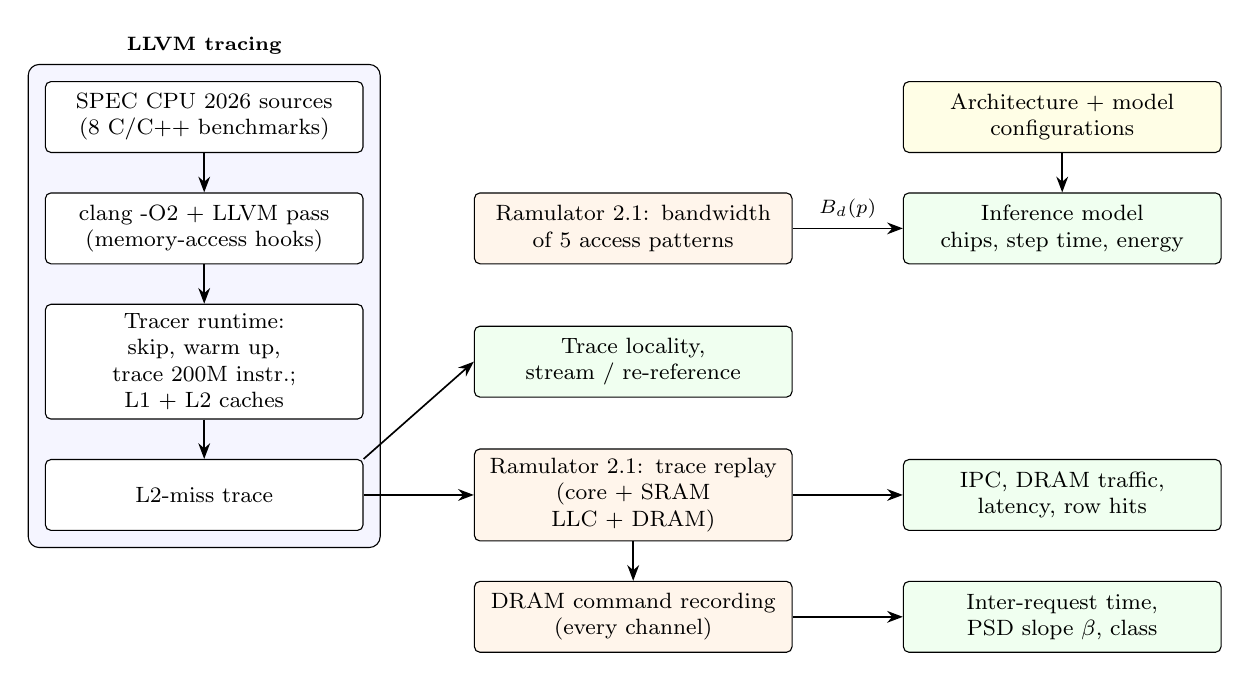
\begin{tikzpicture}[
  font=\footnotesize,
  box/.style={draw, rounded corners=2pt, align=center, minimum height=9mm, text width=38mm, fill=white},
  grp/.style={draw, rounded corners=4pt, inner sep=6pt},
  arr/.style={-{Stealth[length=2mm]}, semithick},
  node distance=5mm and 7mm]
% SPEC tracing column
\node[box] (spec) {SPEC CPU 2026 sources\\(8 C/C++ benchmarks)};
\node[box, below=of spec] (pass) {clang -O2 + LLVM pass\\(memory-access hooks)};
\node[box, below=of pass] (rt) {Tracer runtime: skip, warm up,\\trace 200M instr.; L1 + L2 caches};
\node[box, below=of rt] (trace) {L2-miss trace};
% Ramulator column
\node[box, right=14mm of pass, fill=orange!8] (calib) {Ramulator 2.1: bandwidth\\of 5 access patterns};
\node[box, right=14mm of trace, fill=orange!8] (o3) {Ramulator 2.1: trace replay\\(core + SRAM LLC + DRAM)};
\node[box, below=of o3, fill=orange!8] (rec) {DRAM command recording\\(every channel)};
% Analysis column
\node[box, right=14mm of calib, fill=green!6] (ai) {Inference model\\chips, step time, energy};
\node[box, above=of ai, fill=yellow!10] (cfg) {Architecture + model\\configurations};
\node[box, right=14mm of o3, fill=green!6] (ipc) {IPC, DRAM traffic,\\latency, row hits};
\node[box, right=14mm of rec, fill=green!6] (psd) {Inter-request time,\\PSD slope $\beta$, class};
\node[box, right=14mm of rt, fill=green!6] (loc) {Trace locality,\\stream / re-reference};
\begin{scope}[on background layer]
\node[grp, fill=blue!4, fit=(spec)(trace), label={[font=\scriptsize\bfseries]above:LLVM tracing}] {};
\end{scope}
\draw[arr] (spec) -- (pass);
\draw[arr] (pass) -- (rt);
\draw[arr] (rt) -- (trace);
\draw[arr] (trace) -- (o3);
\draw[arr] (o3) -- (rec);
\draw[arr] (calib) -- node[above, font=\scriptsize]{$B_d(p)$} (ai);
\draw[arr] (cfg) -- (ai);
\draw[arr] (o3) -- (ipc);
\draw[arr] (rec) -- (psd);
\draw[arr] (trace.north east) -- (loc.west);
\end{tikzpicture}
\caption{Framework. Only the memory system differs between architectures: the same operator graphs are used for AI and the same core for SPEC.}
\label{fig:framework}
\end{figure*}

\textbf{DRAM calibration.} Five synthetic access patterns are replayed on each DRAM system and $B_d(p)$ is stored for the inference model. Realistic numbers required a bank-group-aware address mapping (which lifts an HBM3 stream from 51\% to 99\% of pin bandwidth), paired narrow LPDDR5/GDDR6 channels, and HBM's half-rate controller clock in all timing conversions.

\textbf{LLVM tracer.} Our pass plugin instruments the optimized code of each benchmark through SPEC's own build harness, adding a counter at each basic block and a call before every load, store, atomic and memory copy. A small runtime (Algorithm~\ref{alg:trace}) simulates the private caches and writes only L2 misses. Masked vector accesses and uninstrumented library code are not traced (0--13 static masked or gather instructions per binary).

\begin{algorithm}[t]
\caption{Tracer runtime}
\label{alg:trace}
\begin{algorithmic}[1]
\STATE count instructions; skip the first 30B, then warm the caches for 100M
\FORALL{memory accesses in the next 200M instructions}
  \STATE map its page to a physical frame (first-touch order)
  \STATE look it up in the private L1D (48\,KiB) and L2 (2\,MiB) caches
  \IF{it misses in L2}
    \STATE write $\langle$instructions since last miss, address, dirty victim$\rangle$ to the trace
  \ENDIF
\ENDFOR
\end{algorithmic}
\end{algorithm}

\textbf{Replay and characterization.} Each trace is replayed on all seven architectures with 1 core ($N=100$M) and 4 cores ($N=10$M per core; copies of the trace in disjoint address ranges, started together, sharing the LLC and DRAM), giving 112 results. Algorithm~\ref{alg:psd} records every DRAM command of a 60M-instruction replay on the five DRAM-backed systems and analyses the second half of the run time, after the first half has warmed the LLC; a completeness check discards recordings that lost commands. The gaps between consecutive commands, merged over all channels, form the \emph{inter-request time}, the service-side counterpart of the inter-packet arrival time of~\cite{agarwal2025}; zero gaps (commands in the same cycle on different channels) are kept. Its power spectral density $S(f)$ (Welch's method~\cite{welch1967}, Hann window, 50\% overlap; $f$ in cycles per request) is averaged into 32 log-spaced bins and summarised by the least-squares slope $\beta$ of $S(f)\propto 1/f^{\beta}$ over the whole range and over its two halves, split at the log-frequency midpoint, and classified as in~\cite{agarwal2025}: \emph{stationary} (flat, most predictable), \emph{monofractal} (one straight line), \emph{multifractal} (the halves differ by $\ge0.5$; least predictable), plus an \emph{anti-persistent} class of ours for $\beta\le-0.3$. On the trace side, we report each miss's distance to the previous one, the \emph{stream share} (misses to the line after one of the previous 16) and the \emph{re-reference share} (misses to a line already missed).

\begin{algorithm}[t]
\caption{Controller-level characterization}
\label{alg:psd}
\begin{algorithmic}[1]
\FORALL{traces and DRAM-backed architectures}
  \STATE replay 60M instructions on 1 core, recording every DRAM command
  \STATE check that the recording holds every request the DRAM served
  \STATE keep the commands issued in the second half of the run time
  \STATE compute the inter-request times and the average throughput
  \STATE estimate the PSD, fit $\beta$, $\beta_{\mathrm{lo}}$, $\beta_{\mathrm{hi}}$ and assign the class
\ENDFOR
\end{algorithmic}
\end{algorithm}

%=====================================================================
\section{Baselines and Experimental Setup}\label{sec:setup}
%=====================================================================
\textbf{Baselines.} GPU + HBM3 is the baseline of the AI study and CPU + DDR5 that of the SPEC study. A pin-bandwidth (datasheet) roofline is the baseline for the calibration, and published Groq and Cerebras token rates are an external reference for the two SRAM-only systems, whose per-operator overhead and hop latency are the only tuned parameters.

\textbf{Setup.} Ramulator~2.1 is built from source (commit \texttt{7bead6c}); the tracer uses clang/LLVM~23 with \texttt{-O2 -march=x86-64-v3} on SPEC CPU~2026 v1.0.1 \texttt{refrate} inputs, skipping 30B instructions, warming 100M and tracing 200M (LLVM IR instructions). The private caches are a 48\,KiB 12-way L1D and a 2\,MiB 16-way L2 (LRU, write-back); the replay core has a 128-entry window, 32 MSHRs and no prefetcher, and the LLC (LRU, 16--29 ways) has hit latencies from 56 cycles (CPU) to 800 (wafer). Table~\ref{tab:const} lists the inference-model constants. Fifteen unit tests check model sizes, bandwidth bounds, tracer instruction counts, LLC geometry, the PSD classifier on white and $1/f$ noise, and step-time accounting.

%=====================================================================
\section{Results and Performance Analysis}\label{sec:results}
%=====================================================================
\subsection{Achieved DRAM Bandwidth}
Table~\ref{tab:calib} shows that only DDR5, with many banks per channel, holds its bandwidth on every pattern. The fast interfaces lose half or more of it on gathers, so a datasheet roofline overestimates gather bandwidth by up to 4\tmx{}, exactly where paged KV caches and embedding lookups operate.

\begin{table}[t]
\caption{Achieved DRAM Bandwidth in GB/s (\% of Pin), Ramulator 2.1}
\label{tab:calib}
\centering
\footnotesize
\setlength{\tabcolsep}{2.2pt}
\begin{tabular}{@{}lrrrrrr@{}}
\toprule
DRAM & Pin & Stream & RW 2:1 & KV page & Row 256B & Rand 64B\\
\midrule
DDR5 & 307 & 285 (93) & 271 (88) & 284 (93) & 274 (89) & 263 (86)\\
HBM3 & 3,277 & 3,256 (99) & 2,900 (88) & 2,023 (62) & 1,934 (59) & 1,893 (58)\\
HBM4 & 8,192 & 8,107 (99) & 7,247 (88) & 3,914 (48) & 3,784 (46) & 3,736 (46)\\
GDDR6 & 448 & 372 (83) & 303 (68) & 216 (48) & 110 (25) & 108 (24)\\
LPDDR5 & 205 & 198 (97) & 175 (85) & 150 (73) & 93 (45) & 92 (45)\\
\bottomrule
\end{tabular}
\end{table}

\subsection{AI Inference}
Decode is a memory-streaming problem: on every DRAM-based design memory takes 83--100\% of batch-1 decode time, and speed follows achieved bandwidth (Table~\ref{tab:llama}, Fig.~\ref{fig:speedup}). The HBM3 GPU reaches 91\% of its pin-bandwidth bound. SRAM-resident systems are much faster, but only by spreading the model over many chips; their modelled token rates are 0.76--1.9\tmx{} the published Groq and Cerebras figures. The bottleneck therefore moves rather than disappears (Fig.~\ref{fig:breakdown}): the LPU-class system spends 68--79\% of its time on all-reduce latency, and per chip it delivers only 1/12--1/37 of an HBM3 GPU's throughput. Once static power is counted it also uses 5--16\tmx{} the GPU's energy per batch-1 Llama token, even though its memory-access energy is 13--16\tmx{} lower. This all-reduce share is an upper bound, since we assume pure tensor parallelism (Section~\ref{sec:math}). Capacity-bound designs also hit cliffs: when the KV cache outgrows one wafer, throughput per wafer drops 2.3--2.9\tmx{}, while HBM systems degrade smoothly. Note that Fig.~\ref{fig:speedup} compares each system at its own minimum chip count: on Llama-70B at batch 32, one HBM4 GPU (0.79\tmx) is compared with three HBM3 GPUs.

\begin{table}[t]
\caption{Llama-3.1-8B Decode, Batch 1, Context 2,048}
\label{tab:llama}
\centering
\footnotesize
\setlength{\tabcolsep}{2.5pt}
\begin{tabular}{@{}lrrrrrl@{}}
\toprule
Architecture & Chips & Step ms & tok/s & tok/s/chip & vs GPU & Bound\\
\midrule
CPU + DDR5 & 1 & 53.9 & 18.6 & 18.6 & 0.10\tmx & memory\\
GPU + HBM3 & 1 & 5.13 & 194.8 & 194.8 & 1.00\tmx & memory\\
GPU + HBM4 & 1 & 2.31 & 432.9 & 432.9 & 2.22\tmx & memory\\
Mesh + GDDR6 & 1 & 41.4 & 24.2 & 24.2 & 0.12\tmx & memory\\
NPU + LPDDR5 & 1 & 77.0 & 13.0 & 13.0 & 0.07\tmx & memory\\
LPU (SRAM) & 76 & 0.814 & 1,229 & 16.2 & 6.31\tmx & comm.\\
Wafer (SRAM) & 1 & 0.651 & 1,536 & 1,536 & 7.89\tmx & overhead\\
\bottomrule
\end{tabular}
\end{table}

\begin{figure}[t]
\centering
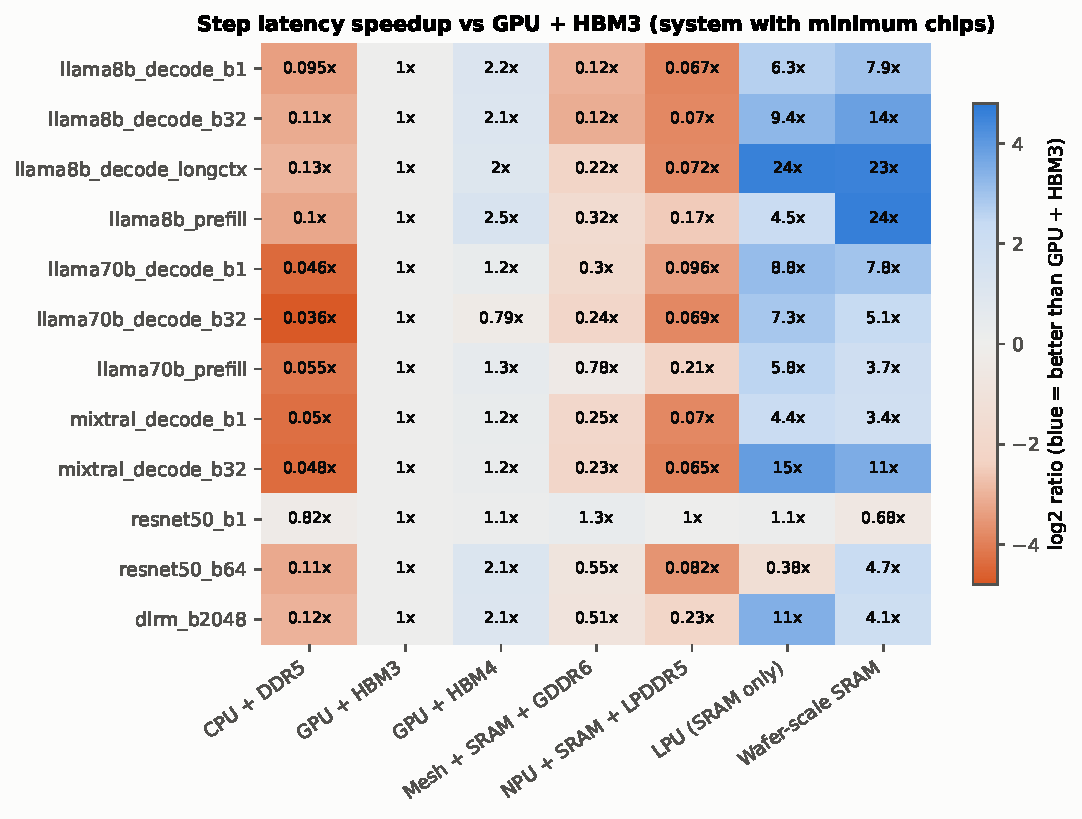
\includegraphics[width=0.95\columnwidth]{figures/03_ai_latency_speedup.pdf}
\caption{Step-latency speedup over GPU + HBM3; each system uses the minimum number of chips that holds the model.}
\label{fig:speedup}
\end{figure}

\begin{figure*}[t]
\centering
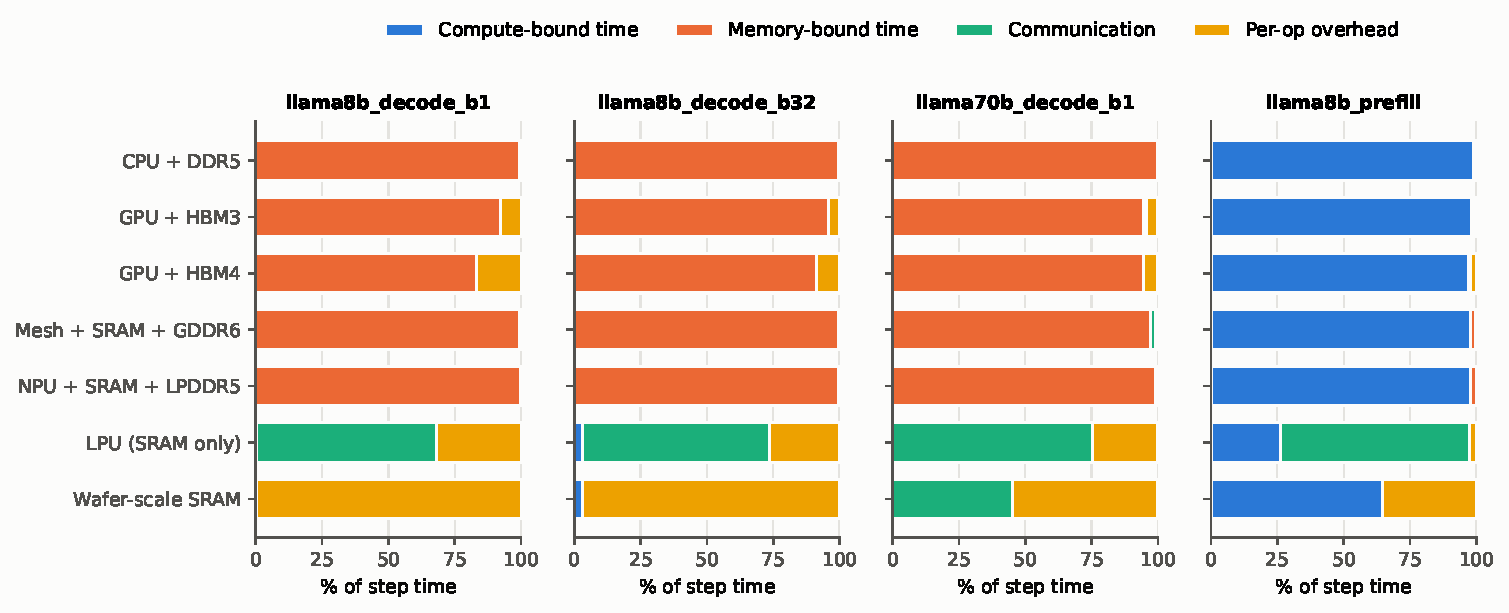
\includegraphics[width=0.72\textwidth]{figures/06_time_breakdown.pdf}
\caption{Where step time goes: DRAM systems are memory-bound in decode and compute-bound in prefill; SRAM-only systems are bound by communication and synchronization.}
\label{fig:breakdown}
\end{figure*}

\subsection{General-Purpose Code}
For seven of the eight benchmarks the hot working set fits in every LLC, so DRAM traffic is almost identical across architectures and IPC follows LLC hit latency instead (Table~\ref{tab:spec}). Large, distant SRAMs hurt pointer-chasing codes most (omnetpp and nest lose 5--7\tmx{} on the wafer). Extra DRAM bandwidth buys nothing: HBM4 matches HBM3, because 4-wide cores with 32 MSHRs and no prefetcher cannot generate enough parallel misses (even 4-core lbm uses 61--67\,GB/s of HBM); throughput-oriented GPUs hide such latencies with many threads, which this study does not model. Capacity helps only bandwidth-heavy lbm, whose DRAM traffic the 208--232\,MiB LLCs cut threefold on 4 cores. The ranking follows SRAM latency, not AI performance: of the two fastest AI systems, the LPU (30\,ns SRAM) is the least affected non-CPU design (0.83\tmx) and the wafer (200\,ns) the most (0.32\tmx).

\begin{table}[t]
\caption{IPC Relative to CPU + DDR5 (1 Core) and Geomeans; APKI on CPU + DDR5}
\label{tab:spec}
\centering
\footnotesize
\setlength{\tabcolsep}{1.9pt}
\begin{tabular}{@{}lrrrrrrrr@{}}
\toprule
Benchmark & APKI & CPU IPC & HBM3 & HBM4 & Mesh & NPU & LPU & Wafer\\
\midrule
stockfish & 0.38 & 3.20 & 0.66 & 0.66 & 0.81 & 0.87 & 0.92 & 0.52\\
sqlite & 0.41 & 3.38 & 0.49 & 0.49 & 0.69 & 0.79 & 0.87 & 0.36\\
omnetpp & 0.20 & 3.22 & 0.28 & 0.28 & 0.47 & 0.61 & 0.71 & 0.18\\
sealcrypto & 0.73 & 3.09 & 0.36 & 0.36 & 0.56 & 0.70 & 0.81 & 0.25\\
nest & 2.04 & 1.86 & 0.23 & 0.23 & 0.41 & 0.56 & 0.71 & 0.15\\
marian & 0.24 & 3.48 & 0.84 & 0.84 & 0.94 & 0.97 & 1.00 & 0.73\\
zstd & 0.54 & 2.80 & 0.47 & 0.47 & 0.66 & 0.77 & 0.88 & 0.33\\
lbm & 43.4 & 1.58 & 0.48 & 0.48 & 0.64 & 0.67 & 0.78 & 0.36\\
\midrule
Geomean, 1 core & & -- & 0.44 & 0.44 & 0.63 & 0.73 & 0.83 & 0.32\\
Geomean, 4 cores & & -- & 0.53 & 0.52 & 0.71 & 0.70 & 0.83 & 0.39\\
\midrule
LLC hit (cycles) & & 56 & 480 & 480 & 240 & 160 & 120 & 800\\
\bottomrule
\end{tabular}
\end{table}

\subsection{Memory Access-Pattern Characterization}
The L2-miss traces (Fig.~\ref{fig:spatial}, Table~\ref{tab:pattern}) fall into four families: streams (marian, sealcrypto), interleaved streams that stay within a page (lbm, the only bandwidth-bound trace), scattered reuse (omnetpp, nest) and sweeps plus scatter (stockfish, sqlite, zstd). Re-referenced misses hit in every LLC, which is why DRAM traffic barely changes across architectures.

\begin{figure*}[t]
\centering
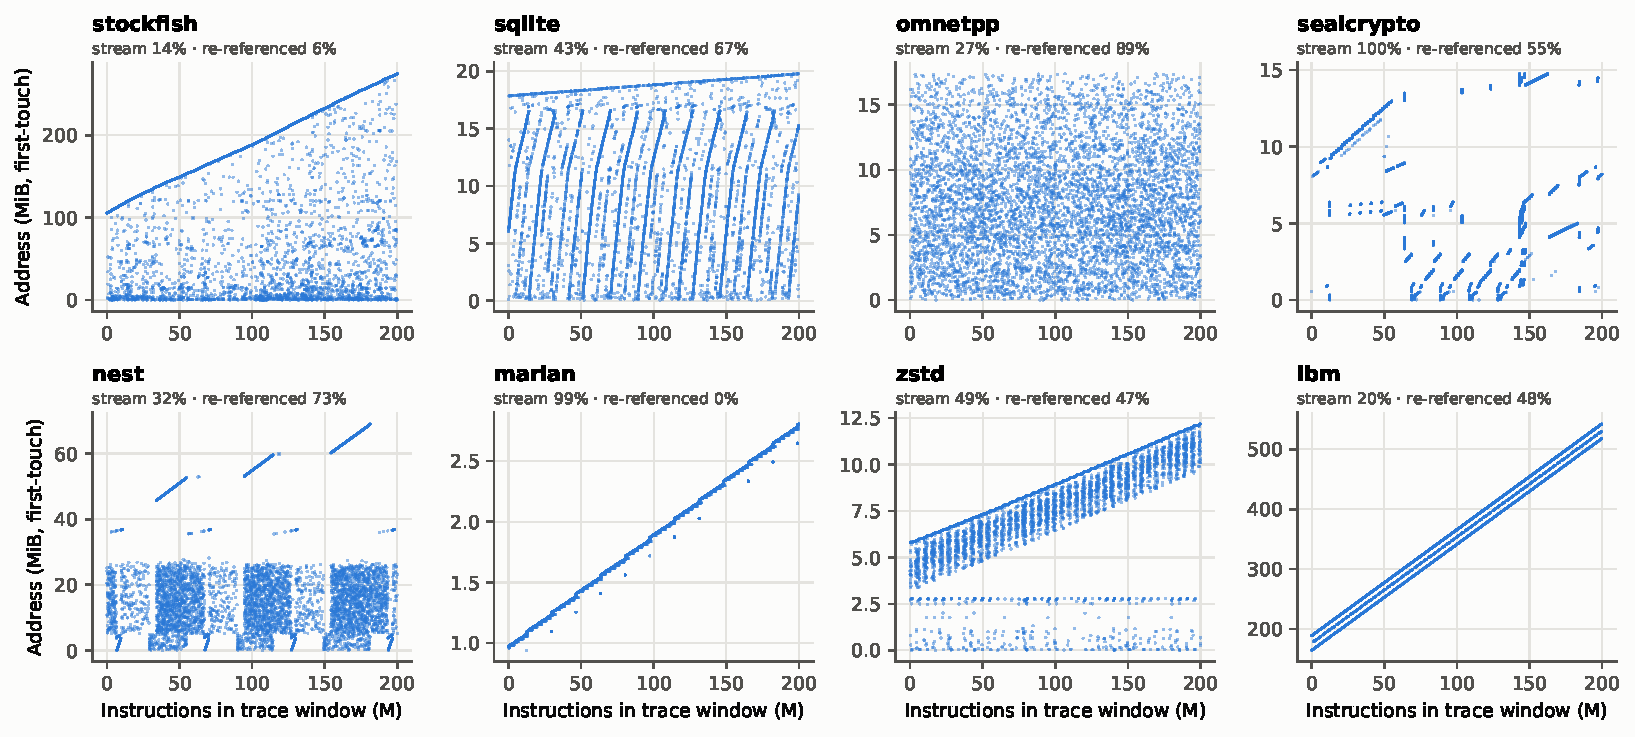
\includegraphics[width=0.72\textwidth]{figures/12_access_spatial.pdf}
\caption{Address of every L2 miss over the 200M-instruction trace window (6,000 samples).}
\label{fig:spatial}
\end{figure*}

\begin{table}[t]
\caption{Trace-Level Access-Pattern Metrics (L2 Misses)}
\label{tab:pattern}
\centering
\footnotesize
\setlength{\tabcolsep}{2.2pt}
\begin{tabular}{@{}lrrrrrrr@{}}
\toprule
Benchmark & MPKI & Mean/med.\ gap & CV & Next & Page & Stream & Re-ref\\
\midrule
stockfish & 0.39 & 2,556 / 2,132 & 1.1 & 12\% & 3\% & 14\% & 6\%\\
sqlite & 2.34 & 428 / 39 & 3.5 & 30\% & 35\% & 43\% & 67\%\\
omnetpp & 5.47 & 183 / 32 & 2.3 & 17\% & 38\% & 27\% & 89\%\\
sealcrypto & 2.63 & 381 / 46 & 29.9 & 80\% & 0\% & 100\% & 55\%\\
nest & 11.47 & 87 / 37 & 1.9 & 19\% & 35\% & 32\% & 73\%\\
marian & 0.15 & 6,667 / 9,168 & 0.6 & 85\% & 0\% & 99\% & 0\%\\
zstd & 1.19 & 841 / 443 & 3.2 & 25\% & 1\% & 49\% & 47\%\\
lbm & 57.89 & 17 / 1 & 5.9 & 0\% & 70\% & 20\% & 48\%\\
\bottomrule
\end{tabular}\\[2pt]
\raggedright\scriptsize Gap in instructions between misses. Next = next 64\,B line; Page = other line in the same 4\,KiB page; Stream = stream share; Re-ref = re-reference share (Section~\ref{sec:method}).
\end{table}

At the memory controllers (Table~\ref{tab:mc}, Fig.~\ref{fig:psd}) the program, not the memory system, sets the shape of the request stream: for five of eight benchmarks $\beta$ varies by at most 0.05 across systems, and 33 of 40 pairs share their benchmark's majority class. Unlike the NoC study~\cite{agarwal2025}, where cache and buffer sizes changed the class, seven of the eight hot sets here fit in every LLC, so the memory system mainly rescales the timing; lbm, which does not fit, is anti-persistent on DDR5 and stationary elsewhere. sealcrypto and omnetpp are largely stationary, stockfish, sqlite and zstd monofractal, and marian and nest multifractal; marian shows a $1/f^2$ low-frequency trend and a period of about 13 requests from its layer-by-layer weight stream. Controller throughput follows IPC rather than DRAM bandwidth: it is highest on CPU + DDR5 and 1.2--3.8\tmx{} lower on the GPUs. Because the analysis window is the second half of the run \emph{time}, it covers different instructions on each system; throughputs are rates, and differences at equal IPC (e.g.\ lbm on HBM3 and HBM4) reflect the sampled program phase.

\begin{table*}[t]
\caption{Memory-Controller Throughput (GB/s) and PSD Slope $\beta$ with Class (S = Stationary, M = Monofractal, MF = Multifractal, AP = Anti-Persistent). Classes also depend on the half-range slopes $\beta_{\mathrm{lo}}$, $\beta_{\mathrm{hi}}$ (not shown), so equal $\beta$ can give different classes.}
\label{tab:mc}
\centering
\footnotesize
\begin{tabular}{@{}lrrrrrcrrrrr@{}}
\toprule
 & \multicolumn{5}{c}{Throughput (GB/s)} & & \multicolumn{5}{c}{$\beta$ (class)}\\
\cmidrule{2-6}\cmidrule{8-12}
Benchmark & DDR5 & HBM3 & HBM4 & GDDR6 & LPDDR5 & & DDR5 & HBM3 & HBM4 & GDDR6 & LPDDR5\\
\midrule
stockfish & 0.44 & 0.31 & 0.31 & 0.37 & 0.39 & & 0.27 M & 0.27 S & 0.27 S & 0.30 M & 0.31 M\\
sqlite & 0.61 & 0.32 & 0.32 & 0.43 & 0.49 & & 0.31 MF & 0.34 M & 0.34 M & 0.32 M & 0.33 M\\
omnetpp & 0.45 & 0.12 & 0.12 & 0.21 & 0.27 & & 0.18 S & 0.18 S & 0.18 S & 0.18 S & 0.20 M\\
sealcrypto & 0.86 & 0.35 & 0.35 & 0.51 & 0.60 & & 0.09 S & 0.05 S & 0.05 S & 0.09 S & 0.10 S\\
nest & 1.95 & 0.61 & 0.60 & 0.98 & 1.17 & & 0.37 MF & 0.12 MF & 0.10 MF & 0.17 MF & 0.42 MF\\
marian & 0.13 & 0.11 & 0.11 & 0.12 & 0.12 & & 1.04 MF & 1.08 MF & 0.98 MF & 0.97 MF & 1.37 MF\\
zstd & 0.45 & 0.21 & 0.21 & 0.30 & 0.34 & & 0.53 M & 0.54 MF & 0.54 MF & 0.54 M & 0.55 M\\
lbm & 15.95 & 8.42 & 5.96 & 8.21 & 8.26 & & $-$0.43 AP & $-$0.20 S & $-$0.19 S & $-$0.28 S & $-$0.09 S\\
\bottomrule
\end{tabular}
\end{table*}

\begin{figure*}[t]
\centering
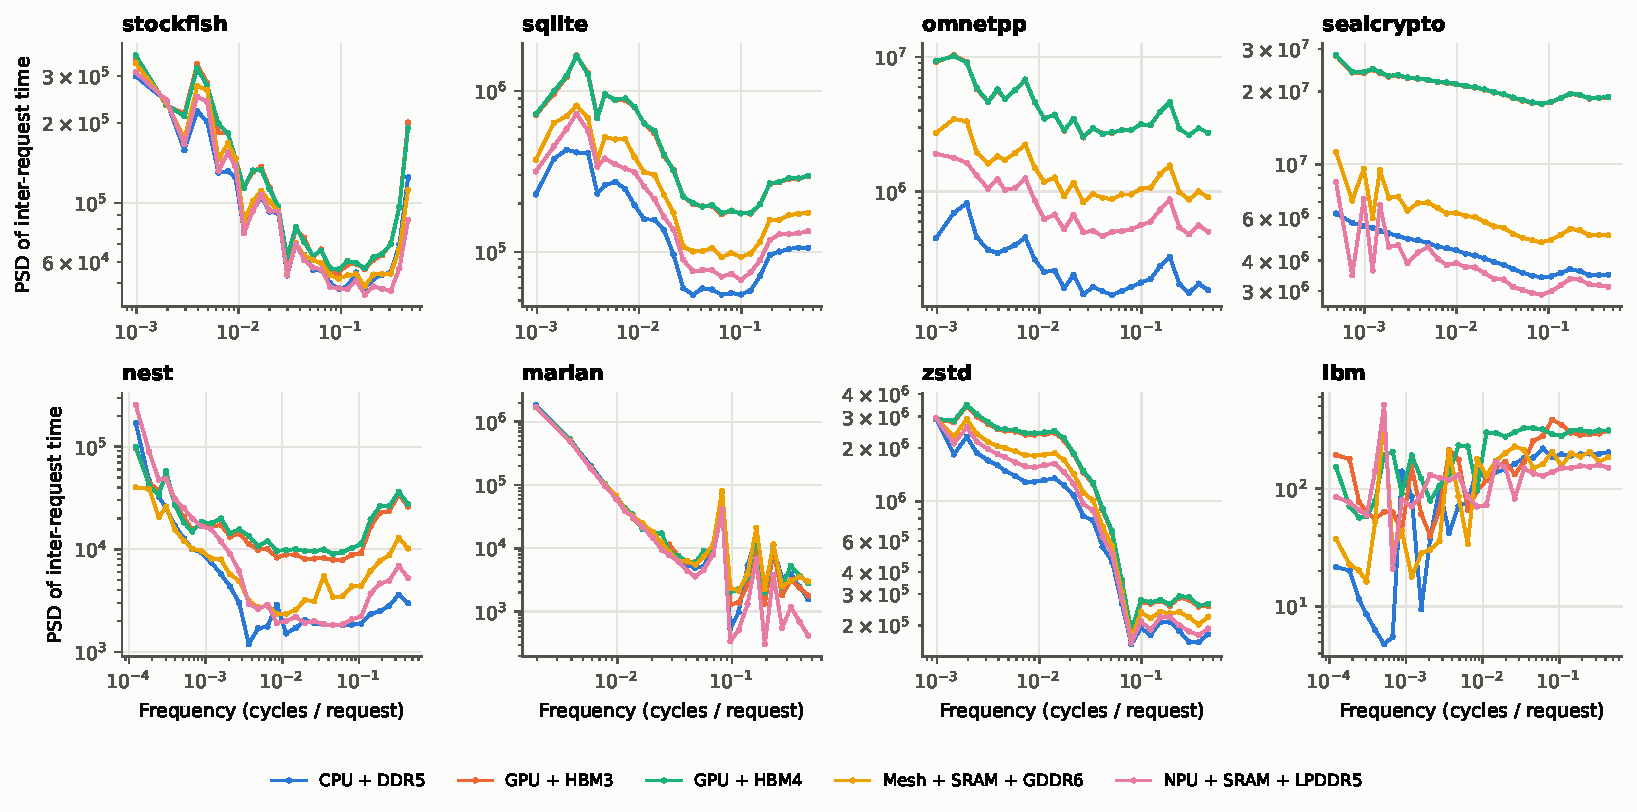
\includegraphics[width=0.72\textwidth]{figures/14_mc_psd.pdf}
\caption{Log-log PSD of the inter-request time at the memory controllers per benchmark and DRAM-backed architecture (cf.~\cite{agarwal2025}); frequency in cycles per request (Nyquist 0.5). marian's $\approx$4,250 requests limit its lowest resolvable frequency.}
\label{fig:psd}
\end{figure*}

Row-buffer locality needs both a spatial pattern and few channels (Fig.~\ref{fig:locality}). Even the most local traces (sealcrypto, lbm) reach only 2--17\% row hits on 128-channel HBM4 but 22--55\% on 16-channel DDR5, because 64\,B interleaving spreads each stream across all channels, so a 4\,KiB page touches each HBM channel at most once: wide AI memory systems turn even sequential streams into row misses.

\begin{figure*}[t]
\centering
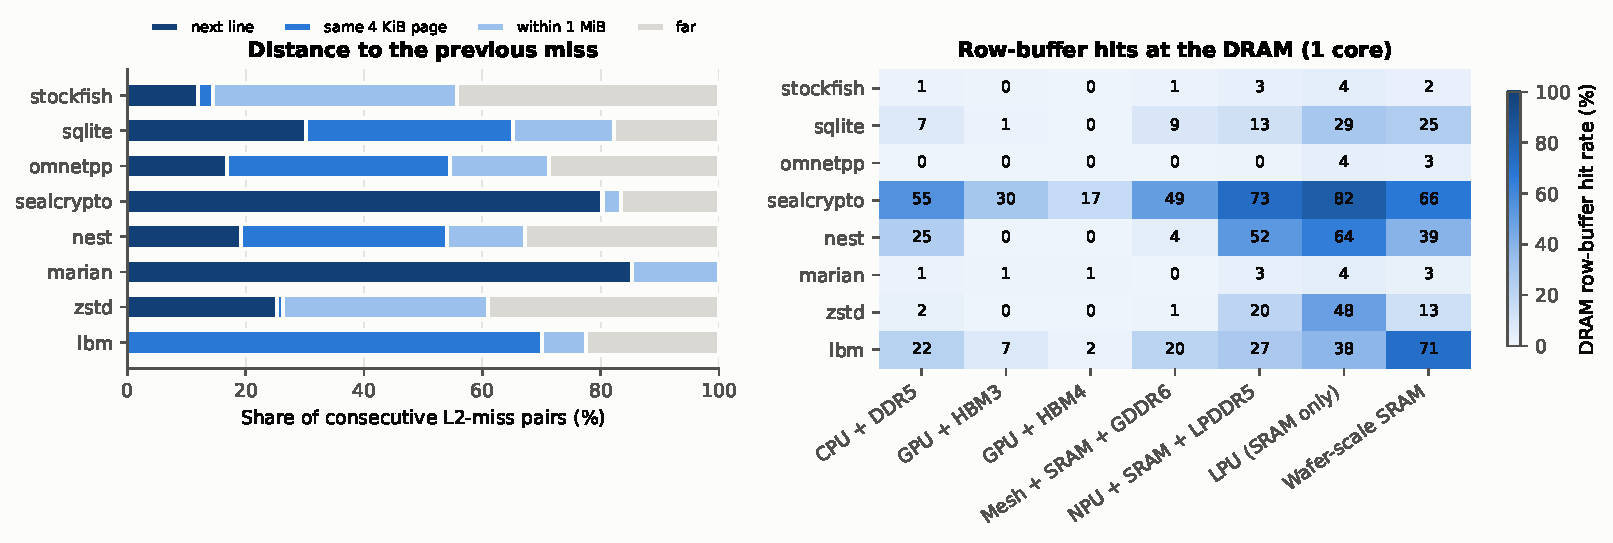
\includegraphics[width=0.72\textwidth]{figures/15_locality.pdf}
\caption{Left: distance of each L2 miss to the previous one. Right: DRAM row-buffer hit rate in the 1-core replays; SRAM-only designs reach a 2-channel host DDR5.}
\label{fig:locality}
\end{figure*}

\textbf{Validation and limitations.} Calibrated bandwidth never exceeds pin bandwidth, and every controller-level replay recorded 100\% of the requests Ramulator served. Parameters are public-specification class values, and the AI model is analytical on top of cycle-accurate DRAM, with pure tensor parallelism and no GPU shared-memory staging. On the SPEC side, each benchmark contributes one 200M-instruction window, the 4-core runs use a short 10M-instruction warm-up with lockstep copies, the core has no prefetcher, and the IPC ratios scale with the assumed SRAM latencies (30--200\,ns). The controller-level PSD merges all channels into one series, which mixes cross-channel interleaving with per-controller burstiness; per-channel spectra are left for future work.

%=====================================================================
\section{Conclusion}\label{sec:conclusion}
%=====================================================================
Inference decode speed tracks \emph{achieved}, not pin, DRAM bandwidth, and fast interfaces lose most of it on gathers. SRAM-only designs buy latency with chips, power and per-chip throughput, and on general-purpose code IPC follows LLC latency rather than DRAM bandwidth, so large, distant on-chip SRAMs cost the most. The shape of the controller request stream is set mainly by the program, and wide memory systems turn even sequential streams into row misses. HBM-based GPUs remain the most balanced choice. Future work includes quantized weights, a prefetching core, and using the PSD class to guide controller scheduling.

\begin{thebibliography}{00}
\bibitem{wulf1995} W. A. Wulf and S. A. McKee, ``Hitting the memory wall: Implications of the obvious,'' \emph{ACM SIGARCH Comput. Archit. News}, vol. 23, no. 1, pp. 20--24, Mar. 1995.
\bibitem{gholami2024} A. Gholami, Z. Yao, S. Kim, C. Hooper, M. W. Mahoney, and K. Keutzer, ``AI and memory wall,'' \emph{IEEE Micro}, vol. 44, no. 3, pp. 33--39, 2024.
\bibitem{choquette2023} J. Choquette, ``NVIDIA Hopper H100 GPU: Scaling performance,'' \emph{IEEE Micro}, vol. 43, no. 3, pp. 9--17, 2023.
\bibitem{vasiljevic2021} J. Vasiljevic \emph{et al.}, ``Compute substrate for Software 2.0,'' \emph{IEEE Micro}, vol. 41, no. 2, pp. 50--55, 2021.
\bibitem{abts2020} D. Abts \emph{et al.}, ``Think fast: A tensor streaming processor (TSP) for accelerating deep learning workloads,'' in \emph{Proc. ACM/IEEE 47th Annu. Int. Symp. Comput. Archit. (ISCA)}, 2020, pp. 145--158.
\bibitem{lie2023} S. Lie, ``Cerebras architecture deep dive: First look inside the hardware/software co-design for deep learning,'' \emph{IEEE Micro}, vol. 43, no. 3, pp. 18--30, 2023.
\bibitem{agarwal2025} S. Agarwal, K. Goel, M. Sinha, and S. Deb, ``Towards improving memory access in large-scale NoC-based systems,'' in \emph{Proc. IEEE Int. Symp. Circuits Syst. (ISCAS)}, 2025, pp. 1--5, doi: 10.1109/ISCAS56072.2025.11043968.
\bibitem{luo2024} H. Luo, Y. C. Tu\u{g}rul, F. N. Bostanc{\i}, A. Olgun, A. G. Ya\u{g}l{\i}k\c{c}{\i}, and O. Mutlu, ``Ramulator 2.0: A modern, modular, and extensible DRAM simulator,'' \emph{IEEE Comput. Archit. Lett.}, vol. 23, no. 1, pp. 112--116, 2024.
\bibitem{pope2023} R. Pope \emph{et al.}, ``Efficiently scaling transformer inference,'' in \emph{Proc. Mach. Learn. Syst. (MLSys)}, vol. 5, 2023.
\bibitem{kwon2023} W. Kwon \emph{et al.}, ``Efficient memory management for large language model serving with PagedAttention,'' in \emph{Proc. 29th ACM Symp. Operating Syst. Princ. (SOSP)}, 2023, pp. 611--626.
\bibitem{zhang2024} H. Zhang, A. Ning, R. B. Prabhakar, and D. Wentzlaff, ``LLMCompass: Enabling efficient hardware design for large language model inference,'' in \emph{Proc. ACM/IEEE 51st Annu. Int. Symp. Comput. Archit. (ISCA)}, 2024, pp. 1080--1096.
\bibitem{bambhaniya2024} A. Bambhaniya \emph{et al.}, ``Demystifying platform requirements for diverse LLM inference use cases,'' arXiv:2406.01698, 2024.
\bibitem{williams2009} S. Williams, A. Waterman, and D. Patterson, ``Roofline: An insightful visual performance model for multicore architectures,'' \emph{Commun. ACM}, vol. 52, no. 4, pp. 65--76, 2009.
\bibitem{jouppi2017} N. P. Jouppi \emph{et al.}, ``In-datacenter performance analysis of a tensor processing unit,'' in \emph{Proc. 44th Annu. Int. Symp. Comput. Archit. (ISCA)}, 2017, pp. 1--12.
\bibitem{kim2016} Y. Kim, W. Yang, and O. Mutlu, ``Ramulator: A fast and extensible DRAM simulator,'' \emph{IEEE Comput. Archit. Lett.}, vol. 15, no. 1, pp. 45--49, 2016.
\bibitem{luk2005} C.-K. Luk \emph{et al.}, ``Pin: Building customized program analysis tools with dynamic instrumentation,'' in \emph{Proc. ACM SIGPLAN Conf. Program. Lang. Des. Implement. (PLDI)}, 2005, pp. 190--200.
\bibitem{limaye2018} A. Limaye and T. Adegbija, ``A workload characterization of the SPEC CPU2017 benchmark suite,'' in \emph{Proc. IEEE Int. Symp. Perform. Anal. Syst. Softw. (ISPASS)}, 2018, pp. 149--158.
\bibitem{lattner2004} C. Lattner and V. Adve, ``LLVM: A compilation framework for lifelong program analysis \& transformation,'' in \emph{Proc. Int. Symp. Code Gener. Optim. (CGO)}, 2004, pp. 75--86.
\bibitem{bogdan2010} P. Bogdan, M. Kas, R. Marculescu, and O. Mutlu, ``QuaLe: A quantum-leap inspired model for non-stationary analysis of NoC traffic in chip multi-processors,'' in \emph{Proc. 4th ACM/IEEE Int. Symp. Networks-on-Chip (NOCS)}, 2010, pp. 241--248.
\bibitem{llama3} A. Grattafiori \emph{et al.}, ``The Llama 3 herd of models,'' arXiv:2407.21783, 2024.
\bibitem{jiang2024} A. Q. Jiang \emph{et al.}, ``Mixtral of experts,'' arXiv:2401.04088, 2024.
\bibitem{he2016} K. He, X. Zhang, S. Ren, and J. Sun, ``Deep residual learning for image recognition,'' in \emph{Proc. IEEE Conf. Comput. Vis. Pattern Recognit. (CVPR)}, 2016, pp. 770--778.
\bibitem{naumov2019} M. Naumov \emph{et al.}, ``Deep learning recommendation model for personalization and recommendation systems,'' arXiv:1906.00091, 2019.
\bibitem{spec2026} Standard Performance Evaluation Corporation, ``SPEC CPU 2026,'' v1.0.1. [Online]. Available: \url{https://www.spec.org/}
\bibitem{rixner2000} S. Rixner, W. J. Dally, U. J. Kapasi, P. Mattson, and J. D. Owens, ``Memory access scheduling,'' in \emph{Proc. 27th Annu. Int. Symp. Comput. Archit. (ISCA)}, 2000, pp. 128--138.
\bibitem{thakur2005} R. Thakur, R. Rabenseifner, and W. Gropp, ``Optimization of collective communication operations in MPICH,'' \emph{Int. J. High Perform. Comput. Appl.}, vol. 19, no. 1, pp. 49--66, 2005.
\bibitem{welch1967} P. D. Welch, ``The use of fast Fourier transform for the estimation of power spectra: A method based on time averaging over short, modified periodograms,'' \emph{IEEE Trans. Audio Electroacoust.}, vol. AU-15, no. 2, pp. 70--73, Jun. 1967.
\end{thebibliography}

\end{document}
